%%%%%%%%%%%%%%%%%%%%%%%%%%%%%%%%%%%%%%%%%%%%%%%%%%%%%%%%%%%%%%%%%%%%%%%%%%%%%%%
%% SOCIOL 723 -- Social Statistics II
%% Week 13 -- Causal Machine Learning
%% Wenhao Jiang, Duke University, Fall 2026
%%%%%%%%%%%%%%%%%%%%%%%%%%%%%%%%%%%%%%%%%%%%%%%%%%%%%%%%%%%%%%%%%%%%%%%%%%%%%%%

\documentclass[aspectratio=169,11pt,xcolor=dvipsnames]{beamer}
\mode<presentation>

%% ---- fonts: Latin Modern Roman (the LaTeX default), serif throughout -------
\usepackage[T1]{fontenc}
\usepackage{lmodern}
\usefonttheme{serif}
\renewcommand{\familydefault}{\rmdefault}

%% ---- packages --------------------------------------------------------------
\usepackage{amsmath,amsfonts,amssymb,bm}
\usepackage{graphicx}
\usepackage{booktabs}
\usepackage{array}
\usepackage{tikz}
\usetikzlibrary{arrows.meta,positioning,calc}
\usepackage[english]{babel}

\newcommand{\srcp}[1]{{\scriptsize\color{gray}(#1)}}
\newcommand{\srct}[1]{#1}

\DeclareMathOperator*{\argminop}{arg\,min}
\DeclareMathOperator*{\argmaxop}{arg\,max}
%% \limits forces the subscript underneath even in inline math
\newcommand{\argmin}{\argminop\limits}
\newcommand{\argmax}{\argmaxop\limits}
\DeclareMathOperator{\Cov}{Cov}
\DeclareMathOperator{\Var}{Var}
\DeclareMathOperator{\trace}{tr}
\DeclareMathOperator{\rank}{rank}
\DeclareMathOperator{\plim}{plim}
\newcommand{\indep}{\perp\!\!\!\perp}

%% ---- notation conventions (course-wide) ------------------------------------
\newcommand{\E}{E}
\newcommand{\En}{\mathbb{E}_n}
\newcommand{\R}{\mathbb{R}}
\newcommand{\X}{\bm{X}}
\newcommand{\Y}{\bm{y}}
\newcommand{\Ix}{\bm{I}}
\newcommand{\zero}{\bm{0}}
\newcommand{\bhat}{\hat{\bm{\beta}}}
\newcommand{\dto}{\overset{d}{\longrightarrow}}
\newcommand{\pto}{\overset{p}{\longrightarrow}}
\usetikzlibrary{shapes,decorations.pathmorphing}
\newcommand{\lik}{\mathcal{L}}
\newcommand{\loglik}{\ell}
\newcommand{\Info}{\mathcal{I}}
\newcommand{\SE}{\mathrm{se}}

%% ---- theme -----------------------------------------------------------------
\usetheme{default}
%% thin single-line header: clickable section names, current one highlighted.
%% (miniframes is deliberately not used: one dot per slide wraps to 4 rows here)
\setbeamerfont{section in head/foot}{size=\tiny}
\setbeamertemplate{headline}{%
  \begin{beamercolorbox}[wd=\paperwidth,ht=2.4ex,dp=1.1ex,%
                         leftskip=.3cm,rightskip=.3cm]{section in head/foot}%
    \usebeamerfont{section in head/foot}%
    \insertsectionnavigationhorizontal{.94\paperwidth}{}{}%
  \end{beamercolorbox}%
}

\definecolor{dukeblue}{RGB}{1,33,105}
\definecolor{accent}{RGB}{200,78,0}
\definecolor{softgray}{RGB}{242,242,245}

\setbeamercolor{structure}{fg=dukeblue}
\setbeamercolor{frametitle}{fg=dukeblue,bg=white}
\setbeamercolor{section in head/foot}{fg=white,bg=dukeblue}
\setbeamercolor{section in head/foot shaded}{fg=white!50!dukeblue,bg=dukeblue}
\setbeamercolor{alerted text}{fg=accent}
\setbeamercolor{block title}{fg=white,bg=dukeblue}
\setbeamercolor{block body}{fg=black,bg=softgray}
\setbeamercolor{block title alerted}{fg=white,bg=accent}
\setbeamercolor{block body alerted}{fg=black,bg=softgray}

\setbeamertemplate{footline}[page number]
\setbeamertemplate{navigation symbols}{}
%% continued frames keep the SAME font size and spill onto a new slide
\setbeamertemplate{frametitle continuation}{\ifnum\insertcontinuationcount>1\normalfont\footnotesize\ (cont.)\fi}
\setbeamertemplate{itemize items}[circle]
\setbeamertemplate{blocks}[rounded][shadow=false]
\setbeamerfont{frametitle}{series=\bfseries}
\setbeamerfont{footnote}{size=\scriptsize}
\setbeamerfont{caption}{size=\footnotesize}
\setbeamertemplate{subsection in head/foot}{}
\setbeamertemplate{subsection in head/foot shaded}{}
\setbeamertemplate{caption}[numbered]

\newcommand{\adv}{\,\raisebox{0.6pt}{\textcolor{accent}{$\bigstar$}}}
%% marker for essential material every student must understand (examinable core)
\definecolor{corestar}{RGB}{0,83,155}
\newcommand{\core}{\,\raisebox{0.6pt}{\textcolor{corestar}{$\bigstar$}}}

\setbeamertemplate{section page}{%
  \begin{centering}\vfill
  {\usebeamercolor[fg]{structure}\Large\bfseries\insertsectionhead\par}
  \vskip4pt{\color{dukeblue}\rule{0.35\linewidth}{1pt}\par}
  \vfill\end{centering}}
\setbeamertemplate{subsection page}{%
  \begin{centering}\vfill
  {\usebeamercolor[fg]{structure}\large\bfseries\insertsubsectionhead\par}
  \vfill\end{centering}}

\AtBeginDocument{%
  \setlength{\abovedisplayskip}{5pt}%
  \setlength{\belowdisplayskip}{5pt}%
  \setlength{\abovedisplayshortskip}{2pt}%
  \setlength{\belowdisplayshortskip}{3pt}%
}
\setbeamertemplate{frametitle}{%
  \vskip4pt\usebeamerfont{frametitle}\usebeamercolor[fg]{frametitle}%
  \insertframetitle\par\vskip2pt}
\setbeamersize{text margin left=0.75cm, text margin right=0.75cm}

%% ---- title -----------------------------------------------------------------
%% ---- title page: same face as the body (Latin Modern), larger and bold
\setbeamerfont{title}{size*={16}{19},series=\bfseries}
\setbeamerfont{subtitle}{size=\Large,series=\mdseries}
\setbeamerfont{author}{size=\large}
\setbeamerfont{date}{size=\large}
\title[SOCIOL 723]{SOCIOL 723: Social Statistics II\\[-2pt]}
\subtitle{Week 13, Causal Machine Learning\\[-6pt]}
\author[Jiang]{Wenhao Jiang\vspace{-2.5em}}
\institute[Duke]{}
\titlegraphic{
\includegraphics[height=1.3cm]{../Misc/duke_logo.png}}
\date{Department of Sociology, Fall 2026}


\begin{document}

\begin{frame}[plain]
  \titlepage
\end{frame}

\begin{frame}{Today}
  \tableofcontents
  \vskip6pt
  {\footnotesize \core{} $=$ essential, you must understand this \quad\quad \adv{} $=$ for understanding, not examined}
\end{frame}

\begin{frame}{Putting the Two Halves Together\core}
\begin{itemize}\itemsep3pt
  \item \textbf{Weeks 5--11} gave us identification: what must be true for a
        parameter to be causal. Almost every design ended with a nuisance
        function to estimate, a propensity score, an outcome regression, a
        first stage, a conditional trend.
  \item \textbf{Week 12} gave us flexible estimators for exactly such functions,
        which work with many covariates and unknown functional form.
  \item \alert{The obvious move, plug ML into the causal estimator, fails.}
        Today is about why, and what fixes it.
\end{itemize}
\vskip4pt
\begin{block}{The payoff}
We get to relax the functional-form assumptions that identification arguments
have been quietly leaning on all semester, AJR's linear geography control,
the linear propensity score, the additive conditional trend, \emph{without}
giving up $\sqrt n$ inference.
\end{block}
\end{frame}

\begin{frame}{Plan}
\textbf{Goal}: valid $\sqrt n$ inference on a causal parameter when the nuisance
functions are estimated by machine learning, and honest estimates of how effects vary.
\vskip3pt
\begin{enumerate}\itemsep2pt
  \item Why plugging ML into a regression fails: regularization bias, shown in a
        simulation; single versus double selection.
  \item Neyman orthogonality, derived; why the product of errors is what matters.
  \item Cross-fitting and the DML recipe; its variance; the ATE score.
  \item The 401(k) data: OLS, single and double lasso, DML with three learners,
        sensitivity to omitted confounders.
  \item Heterogeneous effects: meta-learners, causal forests, BLP, GATES, RATE,
        policy learning, on the 401(k) data.
  \item Applications in social science: growth mindset, college and low-wage work.
\end{enumerate}
\vskip3pt
{\footnotesize Scripts: \texttt{figs/w13\_sims.R}, \texttt{figs/w13\_401k.R}. Book: \srct{Chernozhukov, Hansen, Kallus, Spindler, and Syrgkanis (2024)}.}
\end{frame}


%%%%%%%%%%%%%%%%%%%%%%%%%%%%%%%%%%%%%%%%%%%%%%%%%%%%%%%%%%%%%%%%%%%%%%%%%%%%%%%
\section[The Problem]{Why Naive ML Fails}
%%%%%%%%%%%%%%%%%%%%%%%%%%%%%%%%%%%%%%%%%%%%%%%%%%%%%%%%%%%%%%%%%%%%%%%%%%%%%%%
\begin{frame}\sectionpage\end{frame}

\begin{frame}{The Partially Linear Model\core}
To see the problem without letting notation hide it, start with the simplest
causal case there is: \emph{one} treatment effect to estimate, but completely
flexible relationships between the controls, the treatment, and the outcome.
That is the \alert{partially linear model}, the workhorse for the rest of the
course:
\begin{align*}
  Y_i &= \theta\, D_i + g(W_i) + \epsilon_i, \qquad \E[\epsilon_i \mid D_i, W_i] = 0 \\
  D_i &= m(W_i) + v_i, \qquad\qquad\ \ \E[v_i \mid W_i] = 0 .
\end{align*}
\vskip3pt
\begin{itemize}\itemsep3pt
  \item $\theta$ is the target: the effect of $D$ holding $W$ fixed, and it is
        assumed constant (relaxed in the last section).
  \item $g$ and $m$ are \alert{nuisance functions}; we do not care about them,
        but we must handle them. They may be highly nonlinear, and $W$ may be
        high-dimensional.
  \item Under conditional ignorability given $W$ (Week 5), $\theta$ is the ATE.
  \item Week 1 solved this when $g$ and $m$ are linear and low-dimensional. The
        question now is what happens when we estimate them with lasso or a forest.
\end{itemize}
\end{frame}

\begin{frame}[allowframebreaks,t]{Attempt 1: Regularization Bias\adv}
The naive approach: fit the partially linear model by ML to get $\hat g$, taking
it from a joint fit of $Y$ on $(D_i, W_i)$ with $D_i$ left \emph{unpenalized} so
that $\hat g$ targets the structural $g$. Then regress $Y_i - \hat g(W_i)$ on
$D_i$.
\begin{align*}
  \hat\theta_{\text{naive}}
  = \frac{\frac1n\sum_i D_i\big(Y_i - \hat g(W_i)\big)}{\frac1n\sum_i D_i^2} .
\end{align*}
Substituting the true model and rescaling,
\begin{align*}
  \sqrt n\big(\hat\theta_{\text{naive}} - \theta\big)
  = \underbrace{\Big(\tfrac1n\textstyle\sum_i D_i^2\Big)^{-1}\tfrac{1}{\sqrt n}\sum_i D_i\epsilon_i}_{\dto\ \mathcal N(0,\Sigma)}
  + \underbrace{\Big(\tfrac1n\textstyle\sum_i D_i^2\Big)^{-1}\tfrac{1}{\sqrt n}\sum_i D_i\big(g(W_i)-\hat g(W_i)\big)}_{\alert{\text{regularization bias}}} .
\end{align*}
\vskip2pt
\begin{itemize}\itemsep2pt
  \item Regularized estimators are \emph{deliberately biased} (Week 12), and
        typically converge more slowly than the parametric $n^{-1/2}$.
  \item Then the second term does not vanish on the $\sqrt n$ scale, the
        nuisance bias is of the same order as, or larger than, the sampling noise
        we are trying to describe.
  \item \alert{The point estimate may be fine; the inference is not.} Confidence
        intervals are centred in the wrong place, and collecting more data does
        not fix it.
  \item \textbf{A trap worth naming.} If you instead regress $Y$ on $W$ alone you
        estimate $\ell(W) = \E[Y\mid W] = \theta\, m(W) + g(W)$, which already
        contains the effect you are after. Subtracting that removes the signal.
        And even with the true $\ell$, regressing $Y - \ell(W)$ on \emph{raw}
        $D_i$ does not recover $\theta$: $D_i$ must be residualized too, which is
        exactly what the next slide does.
\end{itemize}
\end{frame}

\begin{frame}{Attempt 2: Partial Out Both Sides\core}
Frisch--Waugh--Lovell says: residualize $Y$ \emph{and} $D$ on $W$, then regress.
With ML estimates $\hat g$ and $\hat m$,
\begin{align*}
  \tilde Y_i = Y_i - \hat\ell(W_i), \qquad \tilde D_i = D_i - \hat m(W_i),
  \qquad
  \hat\theta = \frac{\frac1n\sum_i \tilde D_i \tilde Y_i}{\frac1n\sum_i \tilde D_i^2} ,
\end{align*}
where $\ell(W) = \E[Y\mid W]$.
\vskip3pt
The bias term now involves the \alert{product} of the two estimation errors:
\begin{align*}
  \text{bias} \approx \sqrt n \cdot \frac1n\sum_i
  \big(m(W_i)-\hat m(W_i)\big)\big(\ell(W_i)-\hat \ell(W_i)\big) .
\end{align*}
\vskip2pt
\alert{This vanishes when
$\|\hat m - m\|_2\,\|\hat\ell - \ell\|_2 = o_p(n^{-1/2})$}, for which it is
sufficient that \emph{each} converge faster than $n^{-1/4}$. Lasso and forests
can do that under sparsity or smoothness assumptions.
\textbf{First-order bias has become second-order.}
\end{frame}

\begin{frame}{Seeing the Bias: a Simulation}
$Y = 0.5\,D + g(W) + \epsilon$, $D = m(W) + v$; random forests for the nuisances;
300 draws \srcp{figs/w13\_sims.R}.
\begin{center}\scriptsize
\renewcommand{\arraystretch}{1.05}
\begin{tabular}{@{}lcccc@{}}
\toprule
 & \multicolumn{2}{c}{A: smooth ($n = 500$)} & \multicolumn{2}{c}{B: very nonlinear ($n = 1{,}000$)} \\
estimator & bias / sd & coverage & bias / sd & coverage \\
\midrule
OLS on $(D, W)$ & $-0.08$ & & $+11.2$ & \\
naive plug-in ($Y - \hat g$ on raw $D$) & $-3.20$ & & $+6.40$ & \\
partialling out, in-sample forests & $+0.11$ & 0.94 & $+3.57$ & 0.04 \\
DML, 5-fold cross-fitting & $+0.28$ & 0.93 & $+3.96$ & 0.01 \\
\midrule
RMSE of $\hat m$, $\hat\ell$ & \multicolumn{2}{c}{0.41, \ 0.35} & \multicolumn{2}{c}{0.43, \ 1.02} \\
\bottomrule
\end{tabular}
\end{center}
\begin{itemize}\itemsep0pt\small
  \item \textbf{A} (Chernozhukov et al.'s Figure 1 design): the naive plug-in is off by
        three sds; partialling out is centred and covers.
  \item \textbf{B}: forests cannot learn $g$ here (RMSE of $\hat\ell$ 1.02); DML is biased too.
        \alert{Orthogonality makes errors multiply; it does not make bad estimates good.}
  \item In-sample forests matched cross-fitting here; learners that overfit more do not.
\end{itemize}
\end{frame}


\begin{frame}{This Is Neyman Orthogonality Again\adv}
The residualized moment condition is
\begin{align*}
  \E\Big[\psi(W_i;\theta,\eta)\Big] = 0, \qquad
  \psi = \Big[\big(Y - \ell(W)\big) - \theta\big(D - m(W)\big)\Big]\,\big(D-m(W)\big) ,
\end{align*}
and it satisfies
\begin{align*}
  \left.\frac{\partial}{\partial\eta}\E\big[\psi(W_i;\theta_0,\eta)\big]\right|_{\eta=\eta_0} = 0 .
\end{align*}
\vskip3pt
\begin{itemize}\itemsep3pt
  \item \alert{You met this property in Week 6}: the AIPW estimator's bias was
        the \emph{product} of the two nuisance errors, so first-order mistakes in
        either one cancel. The partially linear case is the same statement for a
        different moment.
  \item And you derived it in \textbf{Week 1}: FWL is the linear special case, in
        which $\hat m$ is an OLS projection and the ``adaptivity'' of $\hat\beta_1$
        to estimation error in the residuals is exactly orthogonality.
  \item \textbf{The thread of the whole course}: FWL $\to$ AIPW $\to$ DML. One
        idea, three levels of generality.
\end{itemize}
\end{frame}

\begin{frame}{Orthogonality, Derived}
Perturb the nuisances in some direction: $\ell_r = \ell_0 + r\,\delta_\ell$,
$m_r = m_0 + r\,\delta_m$. With $V = D - m_0(W)$ and $\E[V\mid W] = 0$:
\begin{align*}
  \psi_r &= \big[Y - \ell_r - \theta_0(D - m_r)\big](D - m_r)
   && \text{\footnotesize the score} \\
  \frac{\partial}{\partial r}\E[\psi_r]\Big|_{r=0}
  &= \E\big[(-\delta_\ell + \theta_0\delta_m)\,V\big] - \E\big[(Y - \ell_0 - \theta_0 V)\,\delta_m\big]
   && \text{\footnotesize product rule} \\
  &= 0 - \E[\epsilon\,\delta_m] = 0
   && \text{\footnotesize $\E[V\mid W] = 0$, $\E[\epsilon\mid W] = 0$}
\end{align*}
\vskip-3pt
Compare the naive score $\varphi = (Y - \theta D - g(W))\,D$:
\begin{align*}
  \frac{\partial}{\partial r}\E\big[(Y - \theta_0 D - g_0 - r\delta_g)D\big]\Big|_{r=0}
  = -\E[\delta_g(W)\,D] = -\E[\delta_g(W)\,m_0(W)] \neq 0 .
\end{align*}
\vskip-2pt
{\footnotesize A small error in $\hat g$ moves the naive moment at first order; it moves the orthogonal
one only at second order, through products of errors.}
\end{frame}

\begin{frame}{Where the Product Comes From}
Write $V = D - m(W)$, $\epsilon = Y - \ell(W) - \theta_0 V$, and the nuisance errors
$\Delta_m = \hat m - m$, $\Delta_\ell = \hat\ell - \ell$. The cross-fitted score at $\theta_0$ is
\begin{align*}
  \big(Y_i - \hat\ell_i - \theta_0(D_i - \hat m_i)\big)\big(D_i - \hat m_i\big)
  &= \big(\epsilon_i - \Delta_{\ell i} + \theta_0\Delta_{mi}\big)\big(V_i - \Delta_{mi}\big) .
\end{align*}
Multiply out and average:
\begin{align*}
  \tfrac1n\textstyle\sum_i\psi_i
  = \underbrace{\tfrac1n\textstyle\sum \epsilon_i V_i}_{\text{CLT term}}
  \underbrace{- \tfrac1n\textstyle\sum (\Delta_{\ell i} - \theta_0\Delta_{mi})V_i - \tfrac1n\textstyle\sum\epsilon_i\Delta_{mi}}_{\text{mean zero}}
  + \underbrace{\tfrac1n\textstyle\sum (\Delta_{\ell i} - \theta_0\Delta_{mi})\Delta_{mi}}_{\text{product of errors}}
\end{align*}
\begin{itemize}\itemsep2pt
  \item The middle terms have mean zero because $\Delta$ was estimated on \emph{other}
        folds: it is fixed given those folds, while $V_i$ and $\epsilon_i$ have mean
        zero. That is what cross-fitting buys.
  \item The last term is of order $\|\Delta_m\|\,\|\Delta_\ell\| + \|\Delta_m\|^2$; it must be
        $o(n^{-1/2})$, which holds if each error is $o(n^{-1/4})$.
\end{itemize}
\end{frame}


\begin{frame}{Single Selection Versus Double Selection}
{\footnotesize\color{gray}\srct{Belloni, Chernozhukov, and Hansen (2014)}}\vskip1pt
\textbf{Single selection}: lasso of $Y$ on $W$ picks the controls; then OLS of
$Y$ on $D$ and those controls.
\begin{itemize}\itemsep0pt
  \item A confounder that predicts $D$ strongly but $Y$ only moderately is
        likely dropped: its coefficient in the $Y$-lasso is small, and $D$ is not
        there to stand in for it. Omitted-variable bias returns.
\end{itemize}
\vskip2pt
\textbf{Double selection}: union of the controls chosen to predict $Y$ \emph{and}
those chosen to predict $D$; then OLS. A variable important for either equation
is kept: the lasso version of partialling out both sides.
\begin{center}\scriptsize
\renewcommand{\arraystretch}{1.08}
\begin{tabular}{@{}lccc@{}}
\toprule
abortion and crime, 48 states $\times$ 12 years & violent & property & murder \\
\midrule
Donohue and Levitt (2001) & $-0.129$ (0.024) & $-0.091$ (0.018) & $-0.121$ (0.047) \\
all 251 controls & $0.294$ (0.472) & $-0.068$ (0.157) & $0.321$ (1.109) \\
double selection & $-0.087$ (0.181) & $-0.094$ (0.051) & $0.006$ (0.280) \\
\bottomrule
\end{tabular}
\end{center}
{\footnotesize Double selection keeps initial abortion rates and their trends, which predict
abortion with $R^2 \approx 0.9$; the violent-crime and murder effects lose significance.}
\end{frame}


%%%%%%%%%%%%%%%%%%%%%%%%%%%%%%%%%%%%%%%%%%%%%%%%%%%%%%%%%%%%%%%%%%%%%%%%%%%%%%%
\section[DML]{Double Machine Learning}
%%%%%%%%%%%%%%%%%%%%%%%%%%%%%%%%%%%%%%%%%%%%%%%%%%%%%%%%%%%%%%%%%%%%%%%%%%%%%%%
\begin{frame}\sectionpage\end{frame}

\begin{frame}{The Second Ingredient: Cross-Fitting\core}
Orthogonality is not quite enough. If $\hat m$ is fitted on the \emph{same}
observations where it is evaluated, its errors correlate with those units'
outcomes, \alert{overfitting bias}, which orthogonality does not remove.
\vskip3pt
\begin{block}{Cross-fitting}
Split the sample into $K$ folds. For each fold $k$: estimate
$\hat\ell^{(-k)}, \hat m^{(-k)}$ on the \emph{other} folds, and form residuals
only for observations \emph{in} fold $k$. Then pool.
\end{block}
\vskip3pt
\begin{align*}
  \hat\theta_{\text{DML}} =
  \frac{\frac1n\sum_{k}\sum_{i \in \mathcal I_k}
        \big(D_i - \hat m^{(-k)}(W_i)\big)\big(Y_i - \hat\ell^{(-k)}(W_i)\big)}
       {\frac1n\sum_{k}\sum_{i \in \mathcal I_k}\big(D_i - \hat m^{(-k)}(W_i)\big)^2}
\end{align*}
\vskip2pt
This is the same device as cross-validation in Week 12, but used to protect
\emph{inference}, not to select a tuning parameter.
\end{frame}

\begin{frame}[allowframebreaks,t]{The DML Recipe\core}
\begin{enumerate}\itemsep3pt
  \item Split the sample into $K$ folds (typically $K = 5$; split on the
        \emph{independent unit} if data are clustered).
  \item On the training folds, estimate $\hat\ell(W) = \hat\E[Y\mid W]$ and
        $\hat m(W) = \hat\E[D\mid W]$ with any ML method, lasso, random forest,
        boosting, or an ensemble.
  \item On the held-out fold, form residuals $\tilde Y_i$ and $\tilde D_i$.
  \item Pool across folds and regress $\tilde Y$ on $\tilde D$.
  \item With independent observations, the standard error is the usual
        heteroskedasticity-robust one from that final bivariate regression:
        \alert{orthogonality is what makes it valid} despite the ML first stage.
        \emph{With clustered data, keeping clusters intact within folds is not
        enough}, the score variance must also be clustered at the independent unit.
  \item Repeat the whole split several times with different seeds and take the
        median; the answer should not depend on the partition.
\end{enumerate}
\vskip3pt
\srct{Chernozhukov et al.\ (2018)}. In \texttt{R}: \texttt{DoubleML} with
\texttt{mlr3} learners.
\end{frame}

\begin{frame}{The DML Variance}
Write the score as $\psi = (\tilde Y - \theta\tilde D)\tilde D$ with
$\tilde Y = Y - \ell(W)$, $\tilde D = D - m(W)$. A linear score gives a ratio, and a
ratio gives a sandwich:
\begin{align*}
  \hat\theta - \theta_0
  &= \frac{\frac1n\sum_i (\tilde Y_i - \theta_0\tilde D_i)\tilde D_i}{\frac1n\sum_i \tilde D_i^2}
   && \text{\footnotesize subtract $\theta_0$ from the ratio} \\
  \sqrt n(\hat\theta - \theta_0) &\dto N\Big(0,\ \frac{\E[\psi^2]}{J^2}\Big),
  \qquad J = \E[\tilde D^2]
   && \text{\footnotesize CLT on top; LLN below}
\end{align*}
\begin{itemize}\itemsep2pt
  \item The estimate of $\E[\psi^2]/J^2$ is the heteroskedasticity-robust variance
        of the final residual-on-residual regression (Week 2), computed with
        cross-fitted residuals.
  \item Orthogonality is what lets the estimated $\hat\ell, \hat m$ stand in for the
        true ones without adding a term to this variance.
  \item With $S$ repeated splits: take the median estimate, and inflate the
        variance by the spread across splits.
\end{itemize}
\end{frame}

\begin{frame}{The ATE Score: AIPW Is DML}
Binary $D$, no constant-effect assumption: target the ATE with outcome models
$m_d(x) = \E[Y\mid D=d, X=x]$ and propensity $e(x)$ (Week 6):
\begin{align*}
  \psi_i = m_1(X_i) - m_0(X_i)
  + \frac{D_i\,(Y_i - m_1(X_i))}{e(X_i)}
  - \frac{(1-D_i)(Y_i - m_0(X_i))}{1 - e(X_i)} - \theta .
\end{align*}
\begin{itemize}\itemsep3pt
  \item Orthogonal in $(m_0, m_1, e)$: the error is
        $\E\big[(\hat e - e)(\hat m_1 - m_1)/\hat e\big]$ plus the analogous term
        for $m_0$, a product.
  \item With cross-fitted ML for the three functions, this is DML for the
        \textbf{interactive regression model}. It estimates the ATE even when effects vary;
        the partially linear model estimates a variance-weighted average of them.
  \item Weights $1/\hat e$ explode near 0 or 1: check overlap, trim, or
        target the ATT or the overlap-weighted effect (Week 6).
\end{itemize}
\end{frame}

\begin{frame}{DML for Instruments: the Partially Linear IV Model}
$Y = \theta D + g(W) + \epsilon$ with $\E[\epsilon\mid Z, W] = 0$; $D$ endogenous,
$Z$ an instrument valid only conditional on $W$ (Week 7):
\begin{align*}
  \psi = \big[(Y - \ell(W)) - \theta(D - r(W))\big]\big(Z - q(W)\big),
  \qquad
  \hat\theta = \frac{\sum_i (Z_i - \hat q)(Y_i - \hat\ell)}{\sum_i (Z_i - \hat q)(D_i - \hat r)}
\end{align*}
with $\ell, r, q$ the conditional means of $Y, D, Z$ given $W$, cross-fitted.
\begin{itemize}\itemsep3pt
  \item A Wald ratio of residuals: partial $W$ out of $Y$, $D$, and $Z$ by ML, then IV.
  \item Card's proximity instrument (Week 7) is credible only given region,
        urbanicity, and family background; this lets them enter flexibly.
  \item Weak-instrument problems survive: a small $\sum(Z - \hat q)(D - \hat r)$ is
        still a small denominator; Anderson--Rubin logic still applies.
\end{itemize}
\end{frame}

\begin{frame}{Folds, Clusters, and Panels}
\begin{itemize}\itemsep4pt
  \item Cross-fitting assumes the held-out fold is independent of the training
        folds. With students in schools or person-years in a panel, \alert{split by
        school or person}; otherwise the same person's other years leak into
        the nuisance fit and the overfitting bias returns.
  \item The variance must also be clustered at that level (sum the score within
        cluster before squaring).
  \item \textbf{Repeated splits}: the estimate depends on the random partition;
        repeat $S$ times, report the median, and add the between-split spread to
        the variance. The 401(k) estimates use 5 folds $\times$ 5 repetitions.
  \item \textbf{How many folds}: 5 is typical; 2 wastes data in each nuisance fit.
        DML2 (pool the score across folds) is preferred over averaging
        fold-specific estimates.
\end{itemize}
\end{frame}



\begin{frame}[allowframebreaks,t]{What the Theory Requires, and What It Does Not\core}
\begin{columns}[T]
\begin{column}{0.47\textwidth}
\textbf{Requires}
\begin{itemize}\small\itemsep2pt
  \item Conditional ignorability given $W$ (unchanged!).
  \item Overlap: $\hat m(W)$ bounded away from 0 and 1 for binary $D$.
  \item Nuisance convergence fast enough that the \emph{product} of the two
        rates is $o(n^{-1/2})$; each faster than $n^{-1/4}$ is sufficient but not
        necessary. Approximate sparsity for lasso, smoothness for forests.
  \item Orthogonal moment $+$ cross-fitting.
\end{itemize}
\end{column}
\begin{column}{0.49\textwidth}
\textbf{Does not require}
\begin{itemize}\small\itemsep2pt
  \item Correct functional form for $g$ or $m$.
  \item Knowing which of the $p$ covariates matter.
  \item $p \ll n$. High-dimensional $W$ is the point.
  \item Consistent \emph{model selection}, lasso may pick the wrong variables
        and $\hat\theta$ is still fine.
\end{itemize}
\end{column}
\end{columns}
\vskip5pt
\begin{alertblock}{The assumption that does not go away}
\alert{DML does not identify anything.} It is an estimation technology for a
parameter already identified by the arguments of Weeks 5--11. If $W$ omits a
confounder, no amount of machine learning helps.
\end{alertblock}
\end{frame}

\begin{frame}{Running Example: 401(k) Eligibility and Wealth}
\textbf{The question.} Does being eligible for a 401(k) plan raise household
net financial assets? Eligibility is set by the employer, so it is not randomly
assigned: it is plausibly ignorable only after conditioning on income, age, and
other characteristics that predict both job choice and saving
\srcp{Poterba, Venti, and Wise 1994; Chernozhukov et al.\ 2018}.
\vskip3pt
\textbf{The data.} SIPP 1991, 9,915 households (\texttt{hdm::pension}). 37\% eligible.
Controls: age, income, education, family size, married, two earners, defined-benefit
pension, IRA, home owner.
\vskip3pt
\textbf{Why ML}: the confounders enter through income and age in ways no one
would write down; a linear model in nine controls is a strong functional-form claim.
\vskip3pt
\textbf{Plan}: raw gap; OLS; single vs.\ double lasso on a 139-column dictionary;
DML, partially linear and interactive, with lasso, forests, and boosting.
\end{frame}

\begin{frame}{401(k): One Effect, Many Estimators}
Effect of eligibility on net financial assets, dollars (robust se) \srcp{figs/w13\_401k.R}:
\begin{center}\scriptsize
\renewcommand{\arraystretch}{0.95}
\begin{tabular}{@{}llcc@{}}
\toprule
estimator & nuisances & estimate & se \\
\midrule
difference in means & none & 19,559 & 1,413 \\
OLS, 9 linear controls & linear & 5,896 & 1,524 \\
single selection (lasso of $Y$ only) & 9 of 139 terms & 8,099 & \\
double selection & 14 of 139 terms & 8,956 & 1,290 \\
\midrule
DML, partially linear & lasso (139 terms) & 9,609 & 1,343 \\
 & random forest & 8,965 & 1,306 \\
 & boosting & 9,907 & 1,368 \\
DML, interactive (ATE) & lasso & 9,319 & 3,065 \\
 & random forest & 8,022 & 1,214 \\
 & boosting & 8,232 & 1,239 \\
\bottomrule
\end{tabular}
\end{center}
\vskip-4pt
{\footnotesize Flexible adjustment lands near \$8,000--10,000 whatever the learner; Chernozhukov et al.\
(2018) report 9,247 and 8,105 with forests. The partially linear model weights effects by
$\Var(D\mid X)$; the interactive one targets the ATE (lasso's se is large: propensities near 0.04).}
\end{frame}

\begin{frame}{How Robust? Sensitivity for DML}
\srct{Chernozhukov, Cinelli, Newey, Sharma, and Syrgkanis (forthcoming)} extend
Week 6's omitted-variable sensitivity to DML: how strong would an unobserved
confounder have to be?
\vskip3pt
\begin{itemize}\itemsep3pt
  \item Bound the bias by two partial $R^2$'s: how much of the residual variation
        in the outcome, and in the treatment (its Riesz representer), the confounder
        explains, $C_Y^2$ and $C_D^2$.
  \item 401(k), DML with forests: partially linear estimate 9,002 (se 1,394);
        \textbf{robustness value} 5.4\%: a confounder explaining 5.4\% of both
        residual variations would bring the estimate to zero.
  \item A confounder as strong as $C_Y^2 \approx 4\%$, $C_D^2 \approx 3\%$ (their
        benchmark, calibrated on observed variables): bias at most 4,196; bounds
        [4,808; 13,196]. Still positive.
\end{itemize}
\vskip3pt
{\footnotesize Same logic as Cinelli and Hazlett (Week 6), with the treatment equation
replaced by the Riesz representer, which covers the ATE score as well as the partially
linear one.}
\end{frame}


\begin{frame}[allowframebreaks,t]{Where DML Plugs In}
The same two ingredients, an orthogonal score plus cross-fitting, apply to
almost every design in this course:
\begin{center}\footnotesize
\renewcommand{\arraystretch}{1.3}
\begin{tabular}{lll}
\toprule
Design & Nuisance functions & Week \\
\midrule
Partially linear regression & $\E[Y\mid W]$, $\E[D\mid W]$ & 1 \\
Interactive / ATE under CIA (AIPW) & $\E[Y\mid D,W]$, $\Pr(D=1\mid W)$ & 6 \\
Instrumental variables & $\E[Y\mid W]$, $\E[D\mid W]$, $\E[Z\mid W]$ & 7 \\
Regression discontinuity & $\E[Y\mid W]$ within the bandwidth & 9 \\
Conditional DID & outcome trend and propensity, by cohort & 10 \\
\bottomrule
\end{tabular}
\end{center}
\vskip4pt
\begin{itemize}\itemsep2pt
  \item For IV: residualize $Y$, $D$, \emph{and} $Z$ on $W$ using ML, then run
        2SLS on the residuals. This is what lets us replace AJR's ``linear in
        distance from the equator plus continent dummies'' with something
        flexible.
  \item For conditional DID: this is precisely the doubly robust
        Callaway--Sant'Anna estimator from Week 10, with ML nuisances.
\end{itemize}
\end{frame}

\begin{frame}{Recent Directions}
\begin{itemize}\itemsep4pt
  \item \textbf{Automatic debiasing} \srcp{Chernozhukov, Newey, and Singh 2022}: every
        orthogonal score in this lecture is ``plug-in $+$ a weight $\times$ residual''.
        The weight (the Riesz representer: $1/e(X)$ terms for the ATE) can be
        learned directly by lasso, without deriving its formula, for any linear
        functional (average derivatives, policy effects).
  \item \textbf{Deep learning for causal effects}: networks with a shared representation
        of $X$ and one output head per treatment arm, sometimes with a third head
        for the propensity; train, then plug the heads into the AIPW score
        \srcp{Koch et al.\ 2025, a primer for sociologists}.
  \item \textbf{Text and images as confounders}: embeddings (Week 12) enter $W$; the
        orthogonal score makes small errors in those representations second order.
  \item \textbf{Software}: \texttt{DoubleML} (R, Python), \texttt{grf}, and
        \texttt{hdm}; the textbook is \srct{Chernozhukov, Hansen, Kallus, Spindler,
        and Syrgkanis (2024)}.
\end{itemize}
\end{frame}


%%%%%%%%%%%%%%%%%%%%%%%%%%%%%%%%%%%%%%%%%%%%%%%%%%%%%%%%%%%%%%%%%%%%%%%%%%%%%%%
\section[HTE]{Heterogeneous Treatment Effects}
%%%%%%%%%%%%%%%%%%%%%%%%%%%%%%%%%%%%%%%%%%%%%%%%%%%%%%%%%%%%%%%%%%%%%%%%%%%%%%%
\begin{frame}\sectionpage\end{frame}

\begin{frame}{From ATE to CATE\core}
Drop the constant-effect assumption. The target becomes the
\alert{conditional average treatment effect}
\begin{align*}
  \tau(x) = \E\big[Y_i(1) - Y_i(0) \mid X_i = x\big] .
\end{align*}
\vskip3pt
\begin{itemize}\itemsep3pt
  \item Sociologically this is often the substantive question: \emph{for whom}
        does college pay off, \emph{which} neighbourhoods benefit, \emph{who} is
        harmed.
  \item \alert{The naive approach, run subgroup regressions, report the
        significant ones, is a multiple-testing disaster} and does not
        replicate. It is the specification search of Week 2 with more rooms to
        search.
  \item The modern approach: build an orthogonal, doubly robust
        \emph{pseudo-outcome} whose conditional mean is $\tau(x)$, then use ML to
        estimate that conditional mean, with honest sample splitting so that
        the subgroups are not chosen using the same data that tests them.
\end{itemize}
\end{frame}

\begin{frame}{Meta-Learners: Five Ways to Estimate $\tau(x)$}
With $\mu_d(x) = \E[Y\mid D=d, X=x]$ and $e(x) = \Pr(D=1\mid X=x)$:
\begin{center}\scriptsize
\renewcommand{\arraystretch}{1.1}
\begin{tabular}{@{}l>{\raggedright\arraybackslash}p{7.4cm}>{\raggedright\arraybackslash}p{3.4cm}@{}}
\toprule
learner & recipe & weakness \\
\midrule
S & one model $\hat\mu(x, d)$; $\hat\tau(x) = \hat\mu(x,1) - \hat\mu(x,0)$ & regularization can shrink $d$ out \\
T & separate $\hat\mu_1$, $\hat\mu_0$; subtract & errors of two fits add \\
X & impute each unit's effect from the \emph{other} group's model, then smooth, weighted by $e(x)$ \srcp{Künzel et al.\ 2019} & good when groups differ in size \\
R & minimize $\sum_i\big[(Y_i - \hat\ell(X_i)) - (D_i - \hat e(X_i))\tau(X_i)\big]^2$ \srcp{Nie and Wager 2021} & needs orthogonal residuals \\
DR & regress the AIPW pseudo-outcome $\Gamma_i$ on $X_i$ \srcp{Kennedy 2023} & extreme $1/\hat e$ \\
\bottomrule
\end{tabular}
\end{center}
\begin{itemize}\itemsep0pt\small
  \item R and DR are \emph{orthogonal}: their error beyond an oracle is a product,
        $(\hat e - e)(\hat\mu_d - \mu_d)$, as in DML.
  \item The R-learner is Robinson's partialling out with $\theta$ replaced by $\tau(X)$.
\end{itemize}
\end{frame}


\begin{frame}{The Doubly Robust Score as a Pseudo-Outcome\core}
Take the AIPW summand from Week 6, unit by unit:
\begin{align*}
  \Gamma_i = \hat m_1(X_i) - \hat m_0(X_i)
  + \frac{D_i\big(Y_i - \hat m_1(X_i)\big)}{\hat e(X_i)}
  - \frac{(1-D_i)\big(Y_i-\hat m_0(X_i)\big)}{1-\hat e(X_i)} .
\end{align*}
\vskip3pt
\begin{itemize}\itemsep3pt
  \item Its \emph{average} is the AIPW estimate of the ATE; that was Week 6.
  \item With the \emph{true} nuisance functions, its conditional mean is exactly
        the CATE: $\E[\Gamma_i \mid X_i = x] = \tau(x)$. With cross-fitted
        estimates it holds approximately, at a rate governed by the same product
        condition as before.
  \item So: construct $\Gamma_i$ with cross-fitted nuisances, then \alert{regress
        $\Gamma_i$ on $X_i$ by any method you like}.
  \begin{itemize}\itemsep1pt
    \item Regress on a few chosen covariates $\to$ \textbf{group average treatment
          effects} (GATEs) with valid standard errors.
    \item Regress with a forest $\to$ a nonparametric CATE surface.
    \item Regress on a constant $\to$ back to the ATE.
  \end{itemize}
  \item \alert{This one construction unifies the whole section.}
\end{itemize}
\end{frame}

\begin{frame}{Causal Forests\core}
\srct{Wager and Athey (2018)}, \srct{Athey, Tibshirani, and Wager (2019)}: a
random forest whose splits are chosen to maximize \emph{heterogeneity in the
treatment effect} rather than in the outcome.
\vskip3pt
\begin{itemize}\itemsep3pt
  \item \textbf{Honesty}: within each tree, one subsample chooses the splits and a
        \emph{disjoint} subsample estimates the effects in the resulting leaves.
        This is what delivers asymptotic normality and valid pointwise intervals
, without it, leaves are selected \emph{because} they show large
        effects.
  \item \textbf{Local centering}: residualize $Y$ and $D$ on $X$ first (i.e.\
        orthogonalize), exactly as in DML.
  \item Output: an estimate $\hat\tau(x)$ for every unit, with standard errors,
        plus variable-importance measures for \emph{effect} heterogeneity.
  \item \texttt{grf::causal\_forest()}.
\end{itemize}
\end{frame}

\begin{frame}{How a Causal Forest Estimates $\tau(x)$}
A forest defines \alert{weights}: $\alpha_i(x)$ = how often unit $i$ shares a leaf
with the point $x$, averaged over trees. Then solve a local, residualized
regression:
\begin{align*}
  \hat\tau(x) = \frac{\sum_i \alpha_i(x)\,\big(D_i - \hat e(X_i)\big)\big(Y_i - \hat\ell(X_i)\big)}
                     {\sum_i \alpha_i(x)\,\big(D_i - \hat e(X_i)\big)^2}
\end{align*}
\begin{itemize}\itemsep3pt
  \item The partially linear (Robinson) estimator, but weighted toward units near
        $x$: DML made local. With $\alpha_i(x) = 1/n$ it is the DML estimate.
  \item Splits are chosen to make $\hat\tau$ differ most between children
        (a gradient approximation keeps it fast) \srcp{Athey, Tibshirani, and Wager 2019}.
  \item \textbf{Honesty}: half of each tree's subsample chooses the splits, the other
        half fills the leaves. \textbf{Subsampling} (not bootstrap) gives the
        variance for pointwise intervals \srcp{Wager and Athey 2018}.
\end{itemize}
\end{frame}


\begin{frame}{Reporting Heterogeneity Honestly\core}
An estimated $\hat\tau(x)$ that varies is not by itself evidence of
heterogeneity, noise varies too.
\vskip3pt
\begin{itemize}\itemsep3pt
  \item \textbf{Calibration test}: regress the doubly robust scores on
        $\hat\tau(X_i)$ (out of fold). A slope near 1 indicates real, well-calibrated
        heterogeneity; a slope near 0 says your CATE surface is noise.
        \texttt{grf::test\_calibration()}.
  \item \textbf{Sorted group ATEs}: rank units by $\hat\tau$, form quantile
        groups, and report the doubly robust ATE \emph{within each group} using
        held-out data. Then test whether the top and bottom groups differ.
  \item \textbf{Pre-specify} the moderators you care about wherever possible, and
        label exploratory heterogeneity as exploratory.
  \item \alert{Effect heterogeneity is where causal ML is most useful and most
        abused.} The honest-splitting discipline is not optional.
\end{itemize}
\end{frame}

\begin{frame}{Testing for Heterogeneity: BLP and GATES \srcp{Chernozhukov, Demirer, Duflo, and Fernández-Val 2025}}
Given a proxy $S(X)$ for the CATE, built on one half of the data, use the other half:
\begin{align*}
  \textbf{BLP:}\quad &\Gamma_i = \beta_1 + \beta_2\big(S(X_i) - \bar S\big) + \text{error}
   && \text{\footnotesize $\beta_1$: ATE; $\beta_2 = 1$ if $S$ is the true CATE} \\
  \textbf{GATES:}\quad &\gamma_k = \E\big[\Gamma_i \mid S(X_i) \in \text{quintile } k\big]
   && \text{\footnotesize effects in groups sorted by $S$}
\end{align*}
\begin{itemize}\itemsep2pt
  \item $\beta_2 = 0$ means no detectable heterogeneity along $S$; the test is valid even
        if $S$ is a bad estimate (a bad $S$ just has low power).
  \item \textbf{CLAN}: compare covariate means between the most and least affected groups.
  \item Repeat over many splits and report medians (with adjusted $p$-values).
\end{itemize}
\vskip2pt
{\footnotesize India immunization incentives (25 vs.\ 78 villages): ATE 2.8 shots per village per
month; most-affected fifth $+13.2$, least-affected $-8.0$, significantly negative.}
\end{frame}

\begin{frame}{Heterogeneity in the 401(k) Data}
Causal forest on the nine controls; doubly robust scores for every comparison
\srcp{figs/w13\_401k.R}:
\vskip-2pt
\begin{center}
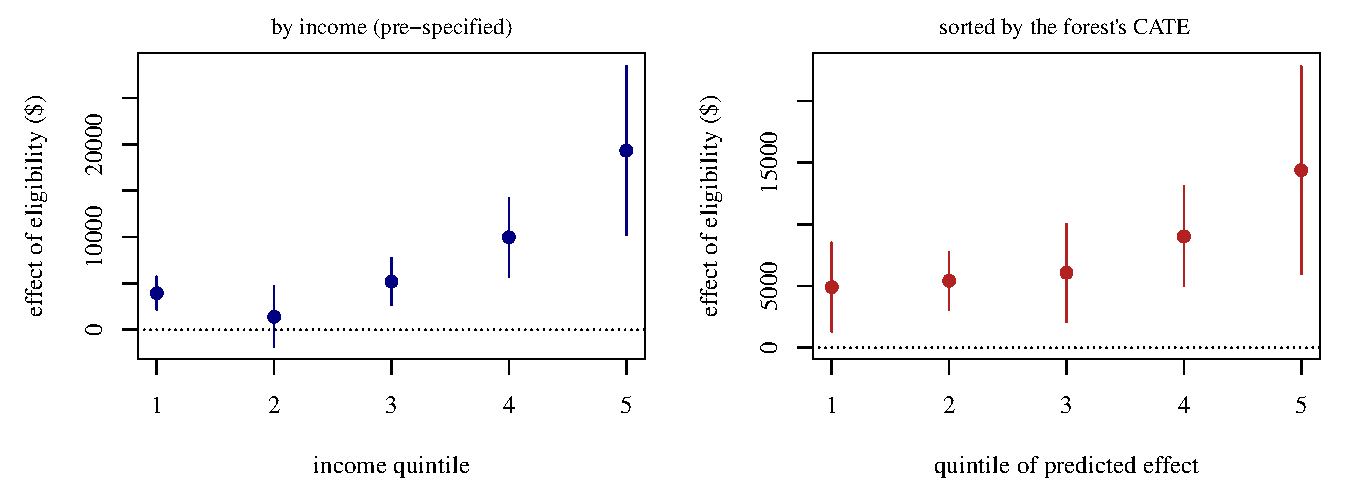
\includegraphics[width=0.66\linewidth]{figs/k401_gates.pdf}
\end{center}
\vskip-10pt
\begin{itemize}\itemsep0pt\small
  \item ATE 7,964 (1,124). Calibration: mean prediction 1.10 (good); differential
        prediction 0.03 ($p = 0.47$): the forest's own ranking carries no detectable signal.
  \item By pre-specified income quintile: 3,946 (904) at the bottom to 19,326 (4,656)
        at the top. Partly scale: dollars of saving rise with income.
  \item RATE on a held-out half: ranking by the forest 1,253 (1,928); by income
        9,661 (5,974). Targeting gains are not established.
\end{itemize}
\end{frame}


\begin{frame}{Should We Target? Rank-Weighted ATEs \srcp{Yadlowsky et al.\ 2025}}
A prioritization rule $S(X)$ ranks units; treat the top share $u$ first.
\begin{align*}
  \text{TOC}(u) &= \E\big[\tau(X)\mid S(X)\ \text{in the top } u\big] - \text{ATE}
   && \text{\footnotesize gain from targeting the top $u$} \\
  \text{RATE} &= \int_0^1 \alpha(u)\,\text{TOC}(u)\,du
   && \text{\footnotesize AUTOC: $\alpha = 1$; Qini: $\alpha(u) = u$}
\end{align*}
\begin{itemize}\itemsep3pt
  \item RATE $> 0$: the rule finds units with larger effects. Estimate $S$ on one
        sample, RATE on another.
  \item Works for any rule: a forest's $\hat\tau(x)$, a risk score, or income.
\end{itemize}
\vskip3pt
\textbf{Policy learning} \srcp{Athey and Wager 2021}: choose a treatment rule
$\pi(x) \in \{0, 1\}$ from a simple class (a depth-2 tree) to maximize
$\frac1n\sum_i (2\pi(X_i) - 1)\,\Gamma_i$; regret shrinks like
$\sqrt{\text{complexity}/n}$. The DR scores again do the work.
\end{frame}

\begin{frame}{Intervals for Individual Effects \srcp{Lei and Candès 2021}}
$\hat\tau(x)$ with a standard error describes the \emph{average} effect among
people like $x$. A person's own effect $Y_i(1) - Y_i(0)$ varies around it.
\vskip3pt
\begin{itemize}\itemsep4pt
  \item Weighted split conformal (Week 12): build a prediction interval for the
        missing $Y_i(1)$ or $Y_i(0)$, reweighting calibration cases by the
        propensity to correct for covariate shift between groups.
  \item Combine the two intervals into an interval for the individual effect,
        with coverage guaranteed if the propensity is known (randomized
        experiments), approximately otherwise.
  \item Typical finding: individual intervals are wide, often covering zero,
        even when the CATE is precisely estimated. Statements about ``who
        benefits'' are about groups.
\end{itemize}
\end{frame}


%%%%%%%%%%%%%%%%%%%%%%%%%%%%%%%%%%%%%%%%%%%%%%%%%%%%%%%%%%%%%%%%%%%%%%%%%%%%%%%
\section[Applications]{Applications}
%%%%%%%%%%%%%%%%%%%%%%%%%%%%%%%%%%%%%%%%%%%%%%%%%%%%%%%%%%%%%%%%%%%%%%%%%%%%%%%
\begin{frame}\sectionpage\end{frame}

\begin{frame}{In the Literature: Growth Mindset in Schools \srcp{Athey and Wager 2019}}
\textbf{The question.} A short online intervention teaches students that
intelligence can grow. For whom does it raise achievement?
\vskip3pt
\textbf{The data.} \alert{Simulated} from a model fit to the National Study of
Learning Mindsets (a randomized study) by the organizers of a 2018 workshop:
10,391 students in 76 schools. The simulated data show selection, so the authors
treat them as observational. A demonstration of method, not a finding about mindsets.
\vskip3pt
\textbf{The design.} A causal forest with propensity and outcome forests for
local centering, clustered by school; heterogeneity checked by the calibration
test and by pre-specified school-level moderators.
\vskip3pt
\begin{center}\small
\renewcommand{\arraystretch}{1.1}
\begin{tabular}{@{}lc@{}}
\toprule
AIPW average effect & 0.247 \ ($\pm 0.04$) \\
above- minus below-median predicted effect & 0.053 \ ($\pm 0.071$) \\
calibration: differential prediction & 0.322 \ (se 0.307, $p = 0.29$) \\
\bottomrule
\end{tabular}
\end{center}
\end{frame}

\begin{frame}{Athey and Wager: What the Forest Could and Could Not Say}
\begin{itemize}\itemsep4pt
  \item The overall effect is clear. The forest's own ranking of students does
        not separate large from small effects: the omnibus test finds no
        heterogeneity it can trust.
  \item One \textbf{pre-specified} school characteristic, the school's average
        fixed mindset, shows credible moderation in a test on school-level DR
        scores ($t = -3.02$, $p = 0.004$); the authors add that it is unclear
        whether it survives controls for other school covariates.
  \item The forest split on that variable often (24\% of depth-weighted
        splits), but splits are not tests: the test came from the DR scores.
  \item Lesson for practice: a CATE surface that varies is not evidence of
        heterogeneity; report the calibration test, and keep a short list of
        moderators chosen before looking.
\end{itemize}
\end{frame}

\begin{frame}{In the Literature: Brand, Xu, Koch, and Geraldo (2021)}
\textbf{The question.} Who benefits most from college, in avoiding low-wage work?
Theories of positive selection (those likeliest to go gain most) and negative
selection (the disadvantaged gain most) predict opposite patterns.
\vskip3pt
\textbf{The data.} NLSY79, ages 14--17 in 1979, completed at least 12th grade:
4,548 respondents. Outcome: share of 1990--2014 spent in low-wage work (below
two thirds of the median hourly wage).
\vskip3pt
\textbf{The design.} \emph{Causal trees} with honest splitting: one half of the
sample grows the tree, the other estimates the effect in each leaf, with
propensity-score matching inside leaves; sensitivity analysis for unobserved
confounding.
\vskip3pt
\textbf{Average effect}: college reduces time in low-wage work by about 18
percentage points (matching), 17 (causal forest).
\end{frame}

\begin{frame}{Brand et al.: Who Gains Most}
The tree's first split is mother's education:
\vskip3pt
\begin{center}\footnotesize
\renewcommand{\arraystretch}{1.05}
\begin{tabular}{@{}lc@{}}
\toprule
leaf & effect of college (pts) \\
\midrule
mother without a high-school degree & $-26$ pts \\
\quad and a large family & $-33$ pts \\
mother high school or more, low income & $-19$ pts \\
\quad father did not attend college & $-21$ pts \\
all respondents & $-17$ to $-18$ pts \\
\bottomrule
\end{tabular}
\end{center}
\vskip3pt
\begin{itemize}\itemsep2pt
  \item Larger effects for the more disadvantaged: \alert{negative selection}, and a
        case for expanding access at the margin where college is least likely.
  \item The leaves are found by the algorithm, not by the authors' hypotheses;
        honest estimation keeps the effects in each leaf from being selected
        because they are large.
\end{itemize}
{\footnotesize Numbers from the 2019 working version; see also \srct{Brand, Zhou, and Xie (2023)} for a review.}
\end{frame}

%%%%%%%%%%%%%%%%%%%%%%%%%%%%%%%%%%%%%%%%%%%%%%%%%%%%%%%%%%%%%%%%%%%%%%%%%%%%%%%
\section[Wrap-Up]{Wrap-Up}
%%%%%%%%%%%%%%%%%%%%%%%%%%%%%%%%%%%%%%%%%%%%%%%%%%%%%%%%%%%%%%%%%%%%%%%%%%%%%%%
\begin{frame}\sectionpage\end{frame}

\begin{frame}{Where This Leaves the Course}
\begin{itemize}\itemsep4pt
  \item \textbf{One idea, three appearances.} FWL (Week 1) $\to$ double
        robustness and Neyman orthogonality (Week 6) $\to$ DML and causal forests
        (today). Each generalizes the last; none replaces identification.
  \item \textbf{ML relaxes functional-form assumptions, not identifying
        assumptions.} That is a real and substantial gain, many published
        identification arguments lean on linearity they never defended, but it
        is a bounded one.
  \item \textbf{The binding constraint is still the design.} A causal forest on a
        confounded comparison estimates heterogeneity in a bias.
\end{itemize}
\vskip4pt
\begin{block}{Next week}
Synthesis, and a review for the final exam.
\end{block}
\end{frame}

\begin{frame}[allowframebreaks,t]{References}
\footnotesize
\begin{itemize}\itemsep2pt
\item Athey, Susan and Guido W. Imbens. 2017. ``The State of Applied Econometrics: Causality and Policy Evaluation.'' \textit{Journal of Economic Perspectives} 31(2): 3--32.
\item Athey, Susan, Julie Tibshirani, and Stefan Wager. 2019. ``Generalized Random Forests.'' \textit{Annals of Statistics} 47(2): 1148--1178.
\item Athey, Susan and Stefan Wager. 2019. ``Estimating Treatment Effects with Causal Forests: An Application.'' \textit{Observational Studies} 5.
\item Athey, Susan and Stefan Wager. 2021. ``Policy Learning with Observational Data.'' \textit{Econometrica} 89(1): 133--161.
\item Bach, Philipp, Malte S. Kurz, Victor Chernozhukov, Martin Spindler, and Sven Klaassen. 2024. ``DoubleML: An Object-Oriented Implementation of Double Machine Learning in R.'' \textit{Journal of Statistical Software} 108(3).
\item Belloni, Alexandre, Victor Chernozhukov, and Christian Hansen. 2014. ``High-Dimensional Methods and Inference on Structural and Treatment Effects.'' \textit{Journal of Economic Perspectives} 28(2): 29--50.
\item Belloni, Alexandre, Victor Chernozhukov, and Christian Hansen. 2014. ``Inference on Treatment Effects after Selection among High-Dimensional Controls.'' \textit{Review of Economic Studies} 81(2): 608--650.
\item Brand, Jennie E., Jiahui Xu, Bernard Koch, and Pablo Geraldo. 2021. ``Uncovering Sociological Effect Heterogeneity Using Tree-Based Machine Learning.'' \textit{Sociological Methodology} 51(2): 189--223.
\item Brand, Jennie E., Xiang Zhou, and Yu Xie. 2023. ``Recent Developments in Causal Inference and Machine Learning.'' \textit{Annual Review of Sociology} 49: 81--110.
\item Chernozhukov, Victor, Denis Chetverikov, Mert Demirer, Esther Duflo, Christian Hansen, Whitney Newey, and James Robins. 2018. ``Double/Debiased Machine Learning for Treatment and Structural Parameters.'' \textit{The Econometrics Journal} 21(1): C1--C68.
\item Chernozhukov, Victor, Carlos Cinelli, Whitney Newey, Amit Sharma, and Vasilis Syrgkanis. Forthcoming. ``Long Story Short: Omitted Variable Bias in Causal Machine Learning.'' \textit{Review of Economics and Statistics}.
\item Chernozhukov, Victor, Mert Demirer, Esther Duflo, and Iván Fernández-Val. 2025. ``Fisher--Schultz Lecture: Generic Machine Learning Inference on Heterogeneous Treatment Effects in Randomized Experiments, with an Application to Immunization in India.'' \textit{Econometrica} 93(4): 1121--1164.
\item Chernozhukov, Victor, Christian Hansen, Nathan Kallus, Martin Spindler, and Vasilis Syrgkanis. 2024. \textit{Applied Causal Inference Powered by ML and AI}. arXiv:2403.02467.
\item Chernozhukov, Victor, Whitney K. Newey, and Rahul Singh. 2022. ``Automatic Debiased Machine Learning of Causal and Structural Effects.'' \textit{Econometrica} 90(3): 967--1027.
\item Kennedy, Edward H. 2023. ``Towards Optimal Doubly Robust Estimation of Heterogeneous Causal Effects.'' \textit{Electronic Journal of Statistics} 17(2): 3008--3049.
\item Koch, Bernard J., Tim Sainburg, Pablo Geraldo, Song Jiang, Yizhou Sun, and Jacob Gates Foster. 2025. ``A Primer on Deep Learning for Causal Inference.'' \textit{Sociological Methods \& Research} 54(2): 397--447.
\item Künzel, Sören R., Jasjeet S. Sekhon, Peter J. Bickel, and Bin Yu. 2019. ``Metalearners for Estimating Heterogeneous Treatment Effects Using Machine Learning.'' \textit{PNAS} 116(10): 4156--4165.
\item Lei, Lihua and Emmanuel J. Candès. 2021. ``Conformal Inference of Counterfactuals and Individual Treatment Effects.'' \textit{Journal of the Royal Statistical Society Series B}: 911--938.
\item Nie, Xinkun and Stefan Wager. 2021. ``Quasi-Oracle Estimation of Heterogeneous Treatment Effects.'' \textit{Biometrika} 108(2): 299--319.
\item Poterba, James M., Steven F. Venti, and David A. Wise. 1994. ``401(k) Plans and Tax-Deferred Saving.'' In \textit{Studies in the Economics of Aging}, edited by D. A. Wise. University of Chicago Press.
\item Robinson, Peter M. 1988. ``Root-N-Consistent Semiparametric Regression.'' \textit{Econometrica} 56(4): 931--954.
\item Wager, Stefan and Susan Athey. 2018. ``Estimation and Inference of Heterogeneous Treatment Effects Using Random Forests.'' \textit{Journal of the American Statistical Association} 113(523): 1228--1242.
\item Yadlowsky, Steve, Scott Fleming, Nigam Shah, Emma Brunskill, and Stefan Wager. 2025. ``Evaluating Treatment Prioritization Rules via Rank-Weighted Average Treatment Effects.'' \textit{Journal of the American Statistical Association} 120(549): 38--51.
\end{itemize}
\end{frame}

\end{document}
